\subsection{Performance comparison with iZ3 and MathSat}\label{performance_oct}

This section discusses a benchmark of interpolation 
generation for the UTVPI theory. Similarly to the previous chapter,
we compare the performance of our tool with respect to the
iZ3 and Mathsat.

\subsubsection{Benchmark description}

The benchmark contains the following parameters:

\begin{itemize}
  \item $l$ stands for a random number of the max value
    of the bounds
  \item $m$ stands for the number of variables allowed
    in the random signature
  \item $n$ stands for the number of inequalities of the
    form: $a_1 x_{k_1} + a_2 x_{k_2} \leq c$
    or $a_1 x_{k_1} - a_2 x_{k_2} \leq c$
    where $a_1, a_2$ are chosen
    uniformly at random from the set of elements
    $\{-1, 0, 1\}$, $k_1, k_2$ are chosen uniformly
    at random from the set of elements 
    $\{1, \dots, n\}$, and $c$ is chosen uniformly
    at random from the set $\{-l, \dots, l\}$
\end{itemize}

We constructed a pair of inconsistent formulas $(A-part, B-part)$
using an identical construction to the benchmark proposed in 
the previous chapter, using two $z3: :solver$ in order to maintain
each $A-part$ and $B-part$ consistent but inconsistent with 
each other. 

\subsubsection{Experimental results}

We designed the problem because the randomness makes it
difficult to come up with trivial solutions. This problem 
was executed $100$ and $10000$ times using the parameters
$(l = 1000, m = 10, n = 5)$ and 
$(l = 10, m = 10, n = 20)$ respectively.

The following graph reports the time needed
by our implementation, iZ3, and the interpolation 
generation algorithm from Mathsat. 
It is well known that both iZ3 and Mathsat does not
compute uniform interpolants for UTVPI. 
Regardless, the benchmark
was used with the purpose to compare their execution time
on normal interpolants.

\begin{figure}
  \centering
  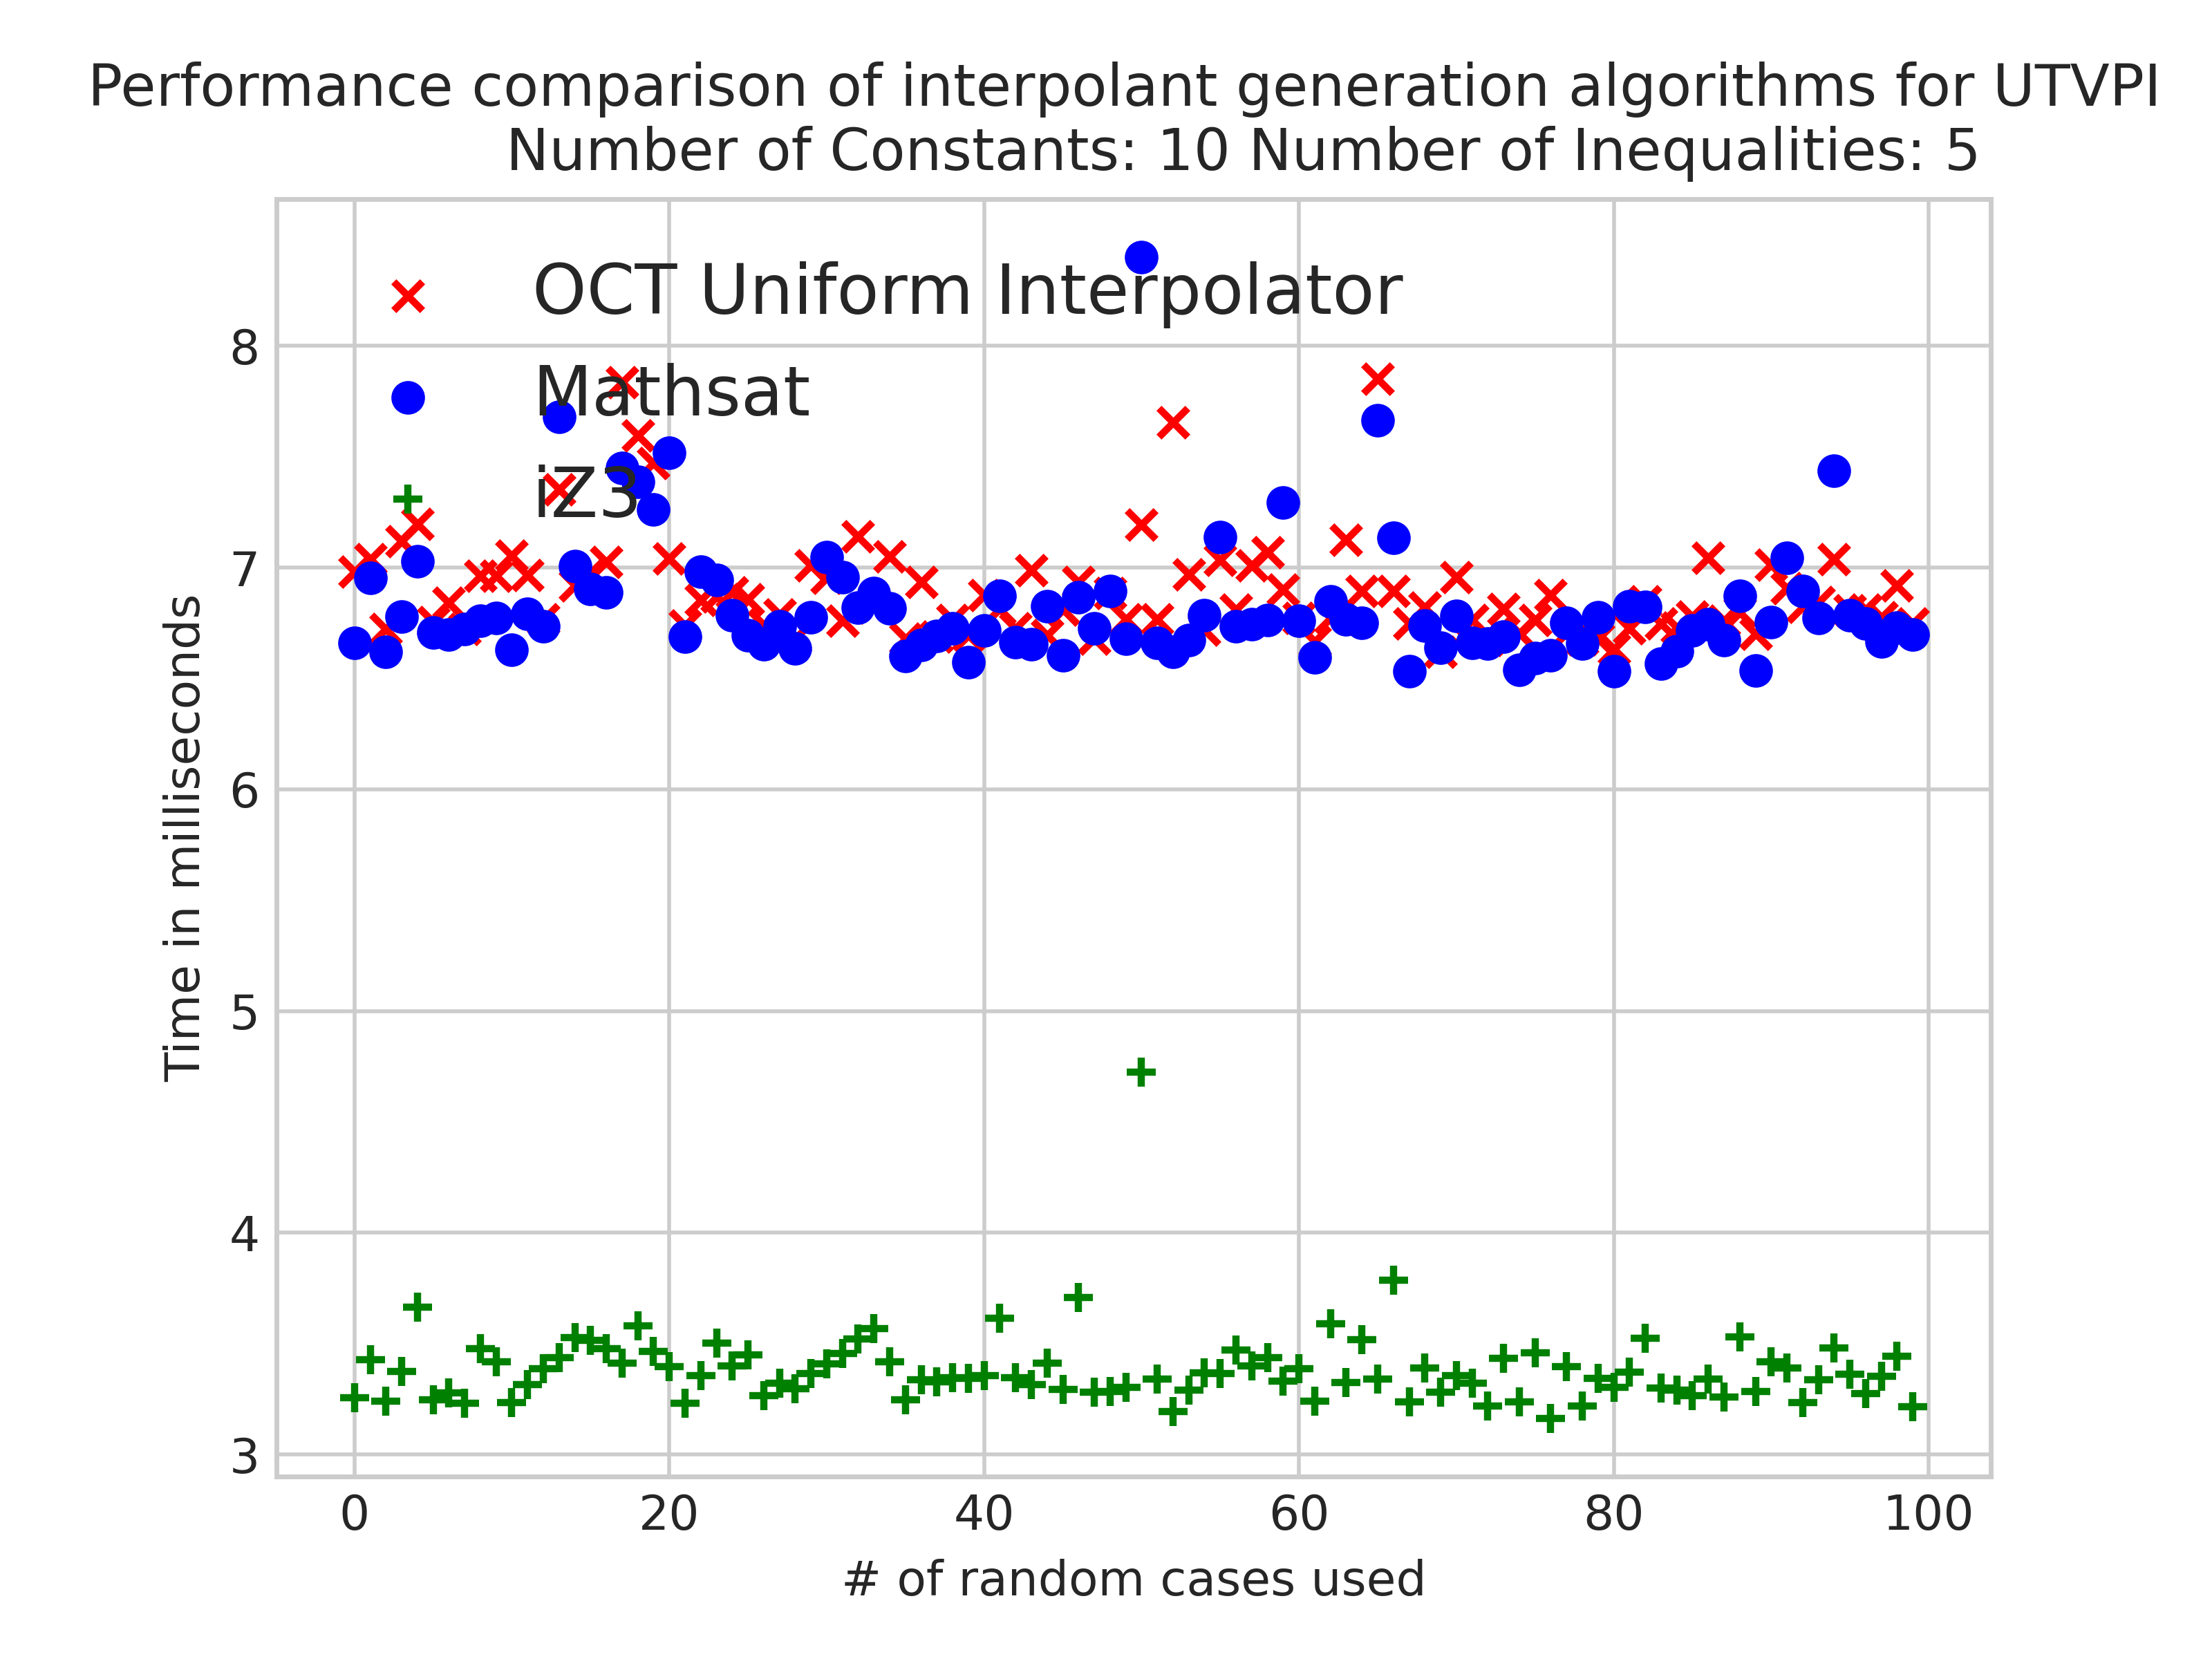
\includegraphics[scale=0.6]{figures/octi_performance_graph_10_5_100}
  \caption{Performance comparison graph of UTVPI interpolant generation
  algorithms for the benchmark (l = 1000, m = 10, n = 5)}
  \label{performance_graph_oct}
\end{figure}

\begin{figure}
  \centering
  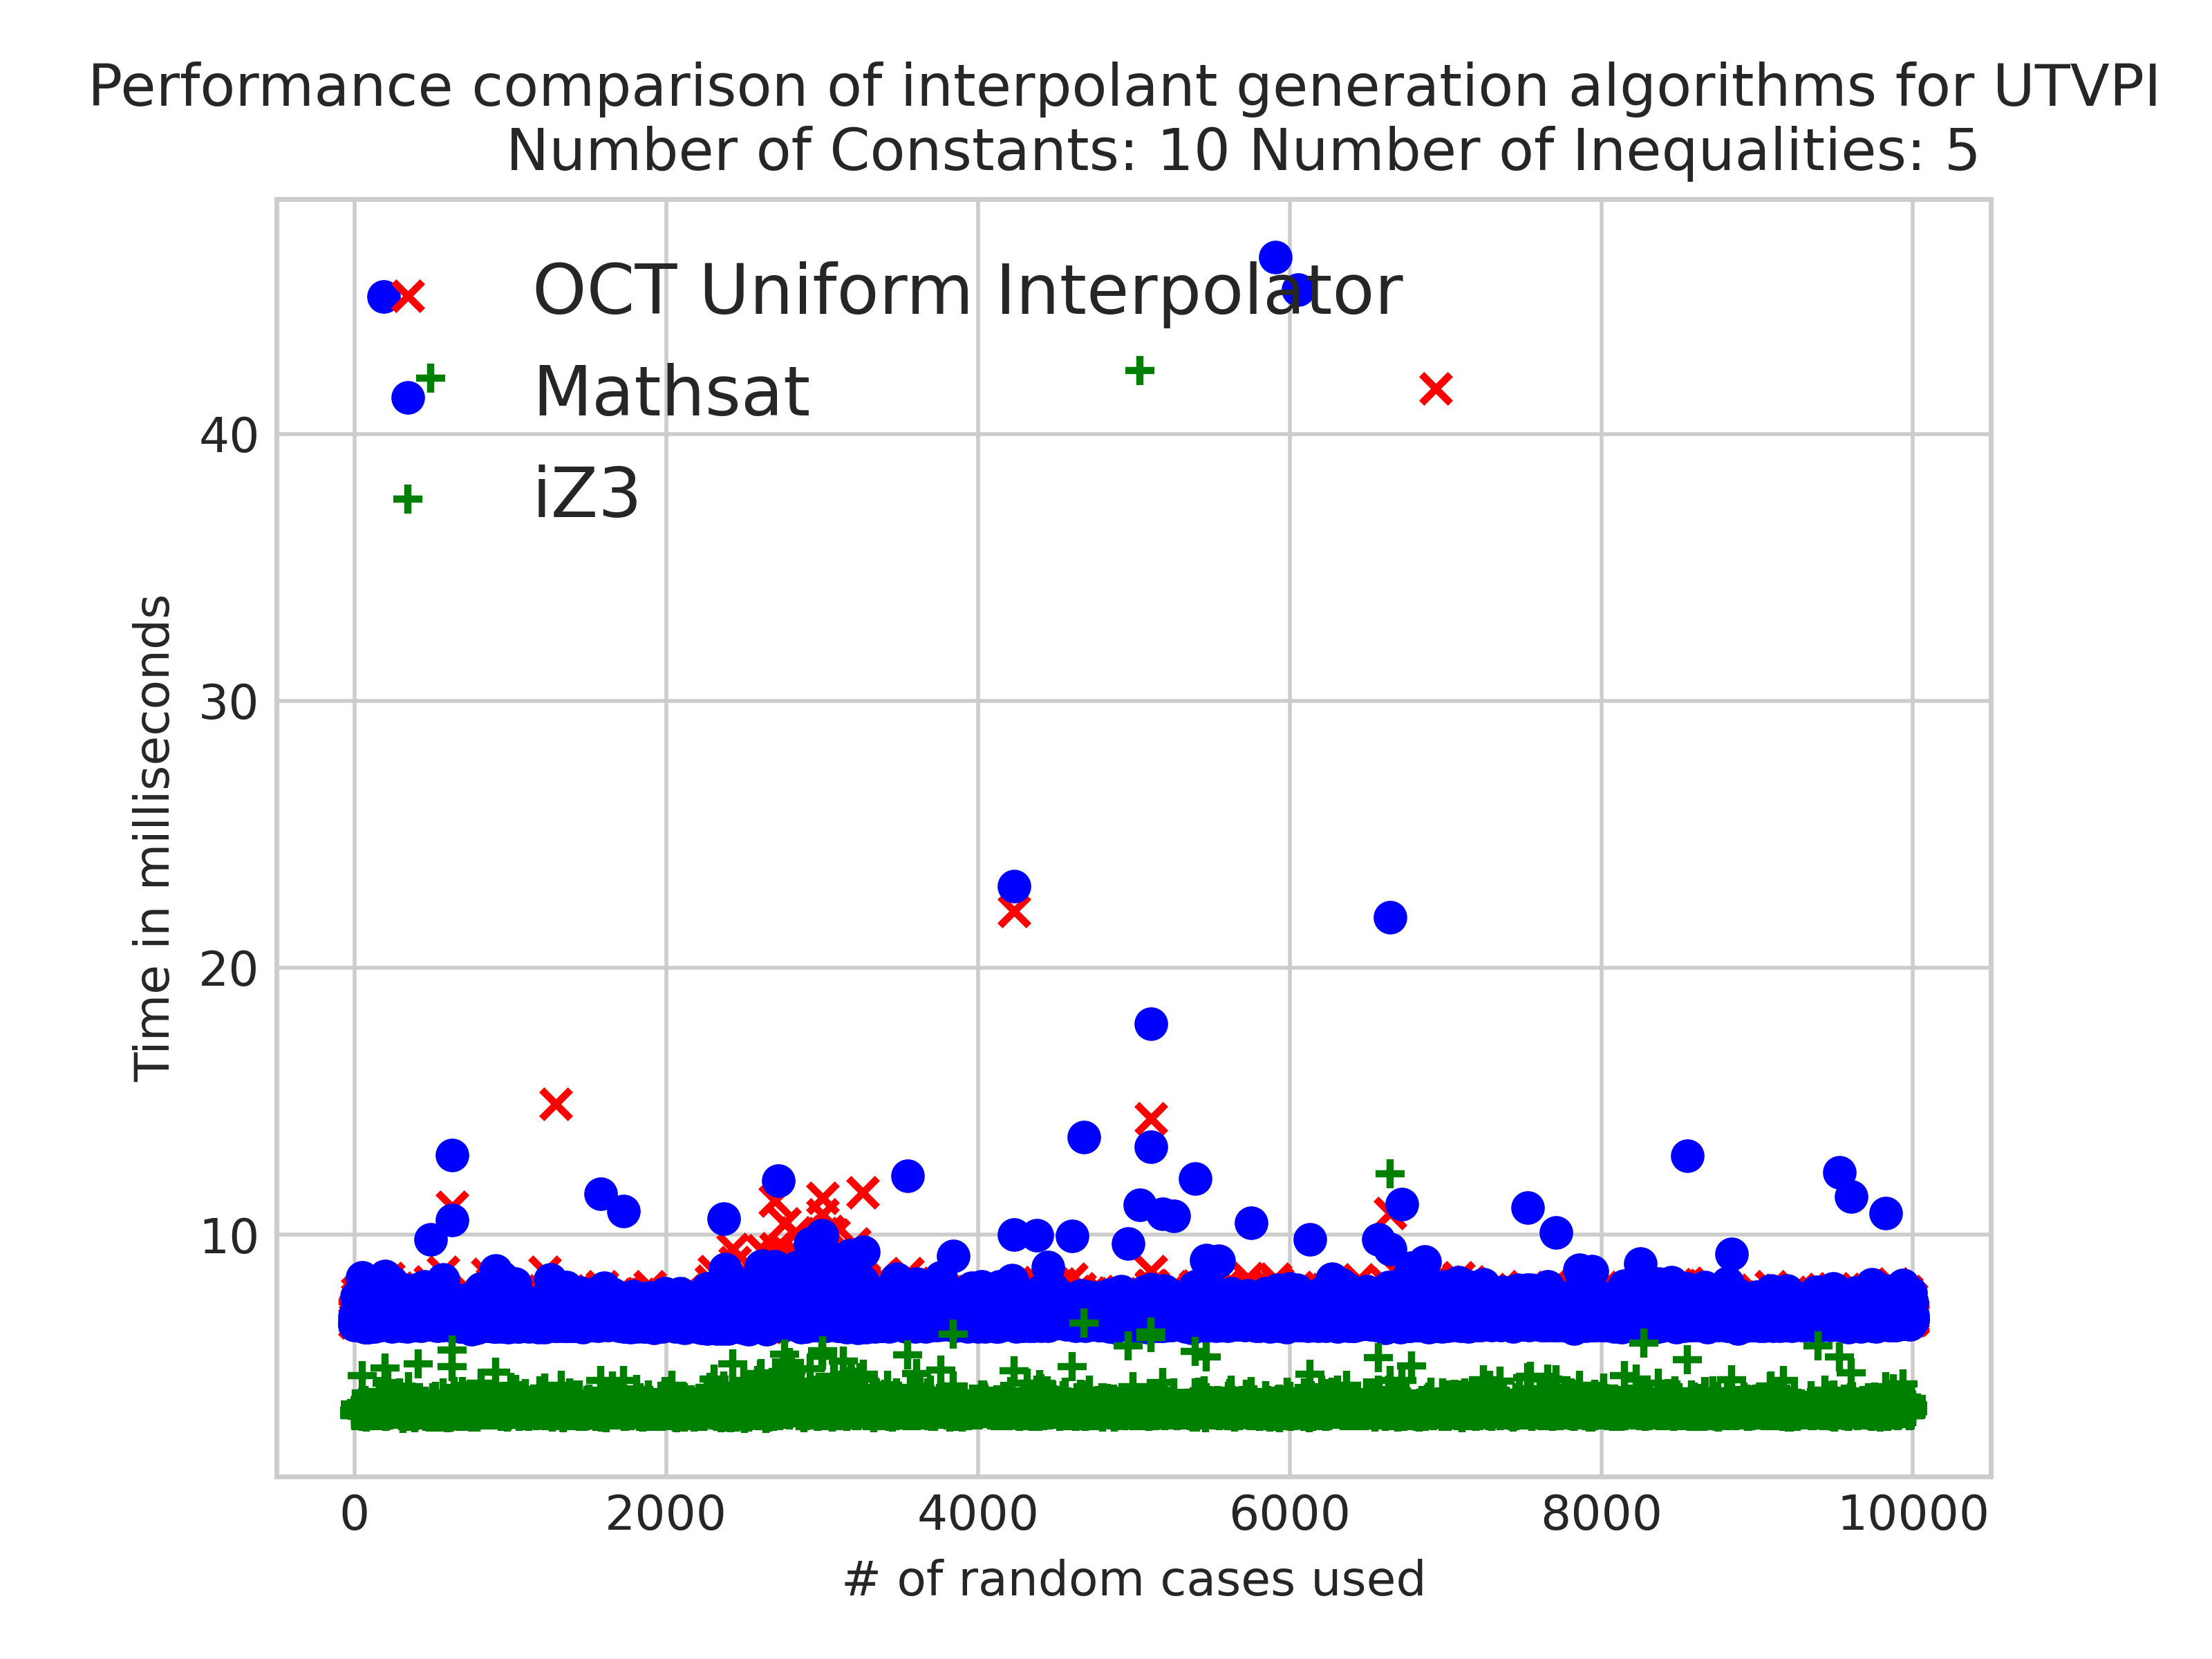
\includegraphics[scale=0.6]{figures/octi_performance_graph_10_5_10000}
  \caption{Performance comparison graph of UTVPI interpolant generation
  algorithms for the benchmark (l = 1000, m = 10, n = 5)} 

  \label{performance_graph_oct_2}
\end{figure}

\begin{figure}
  \centering
  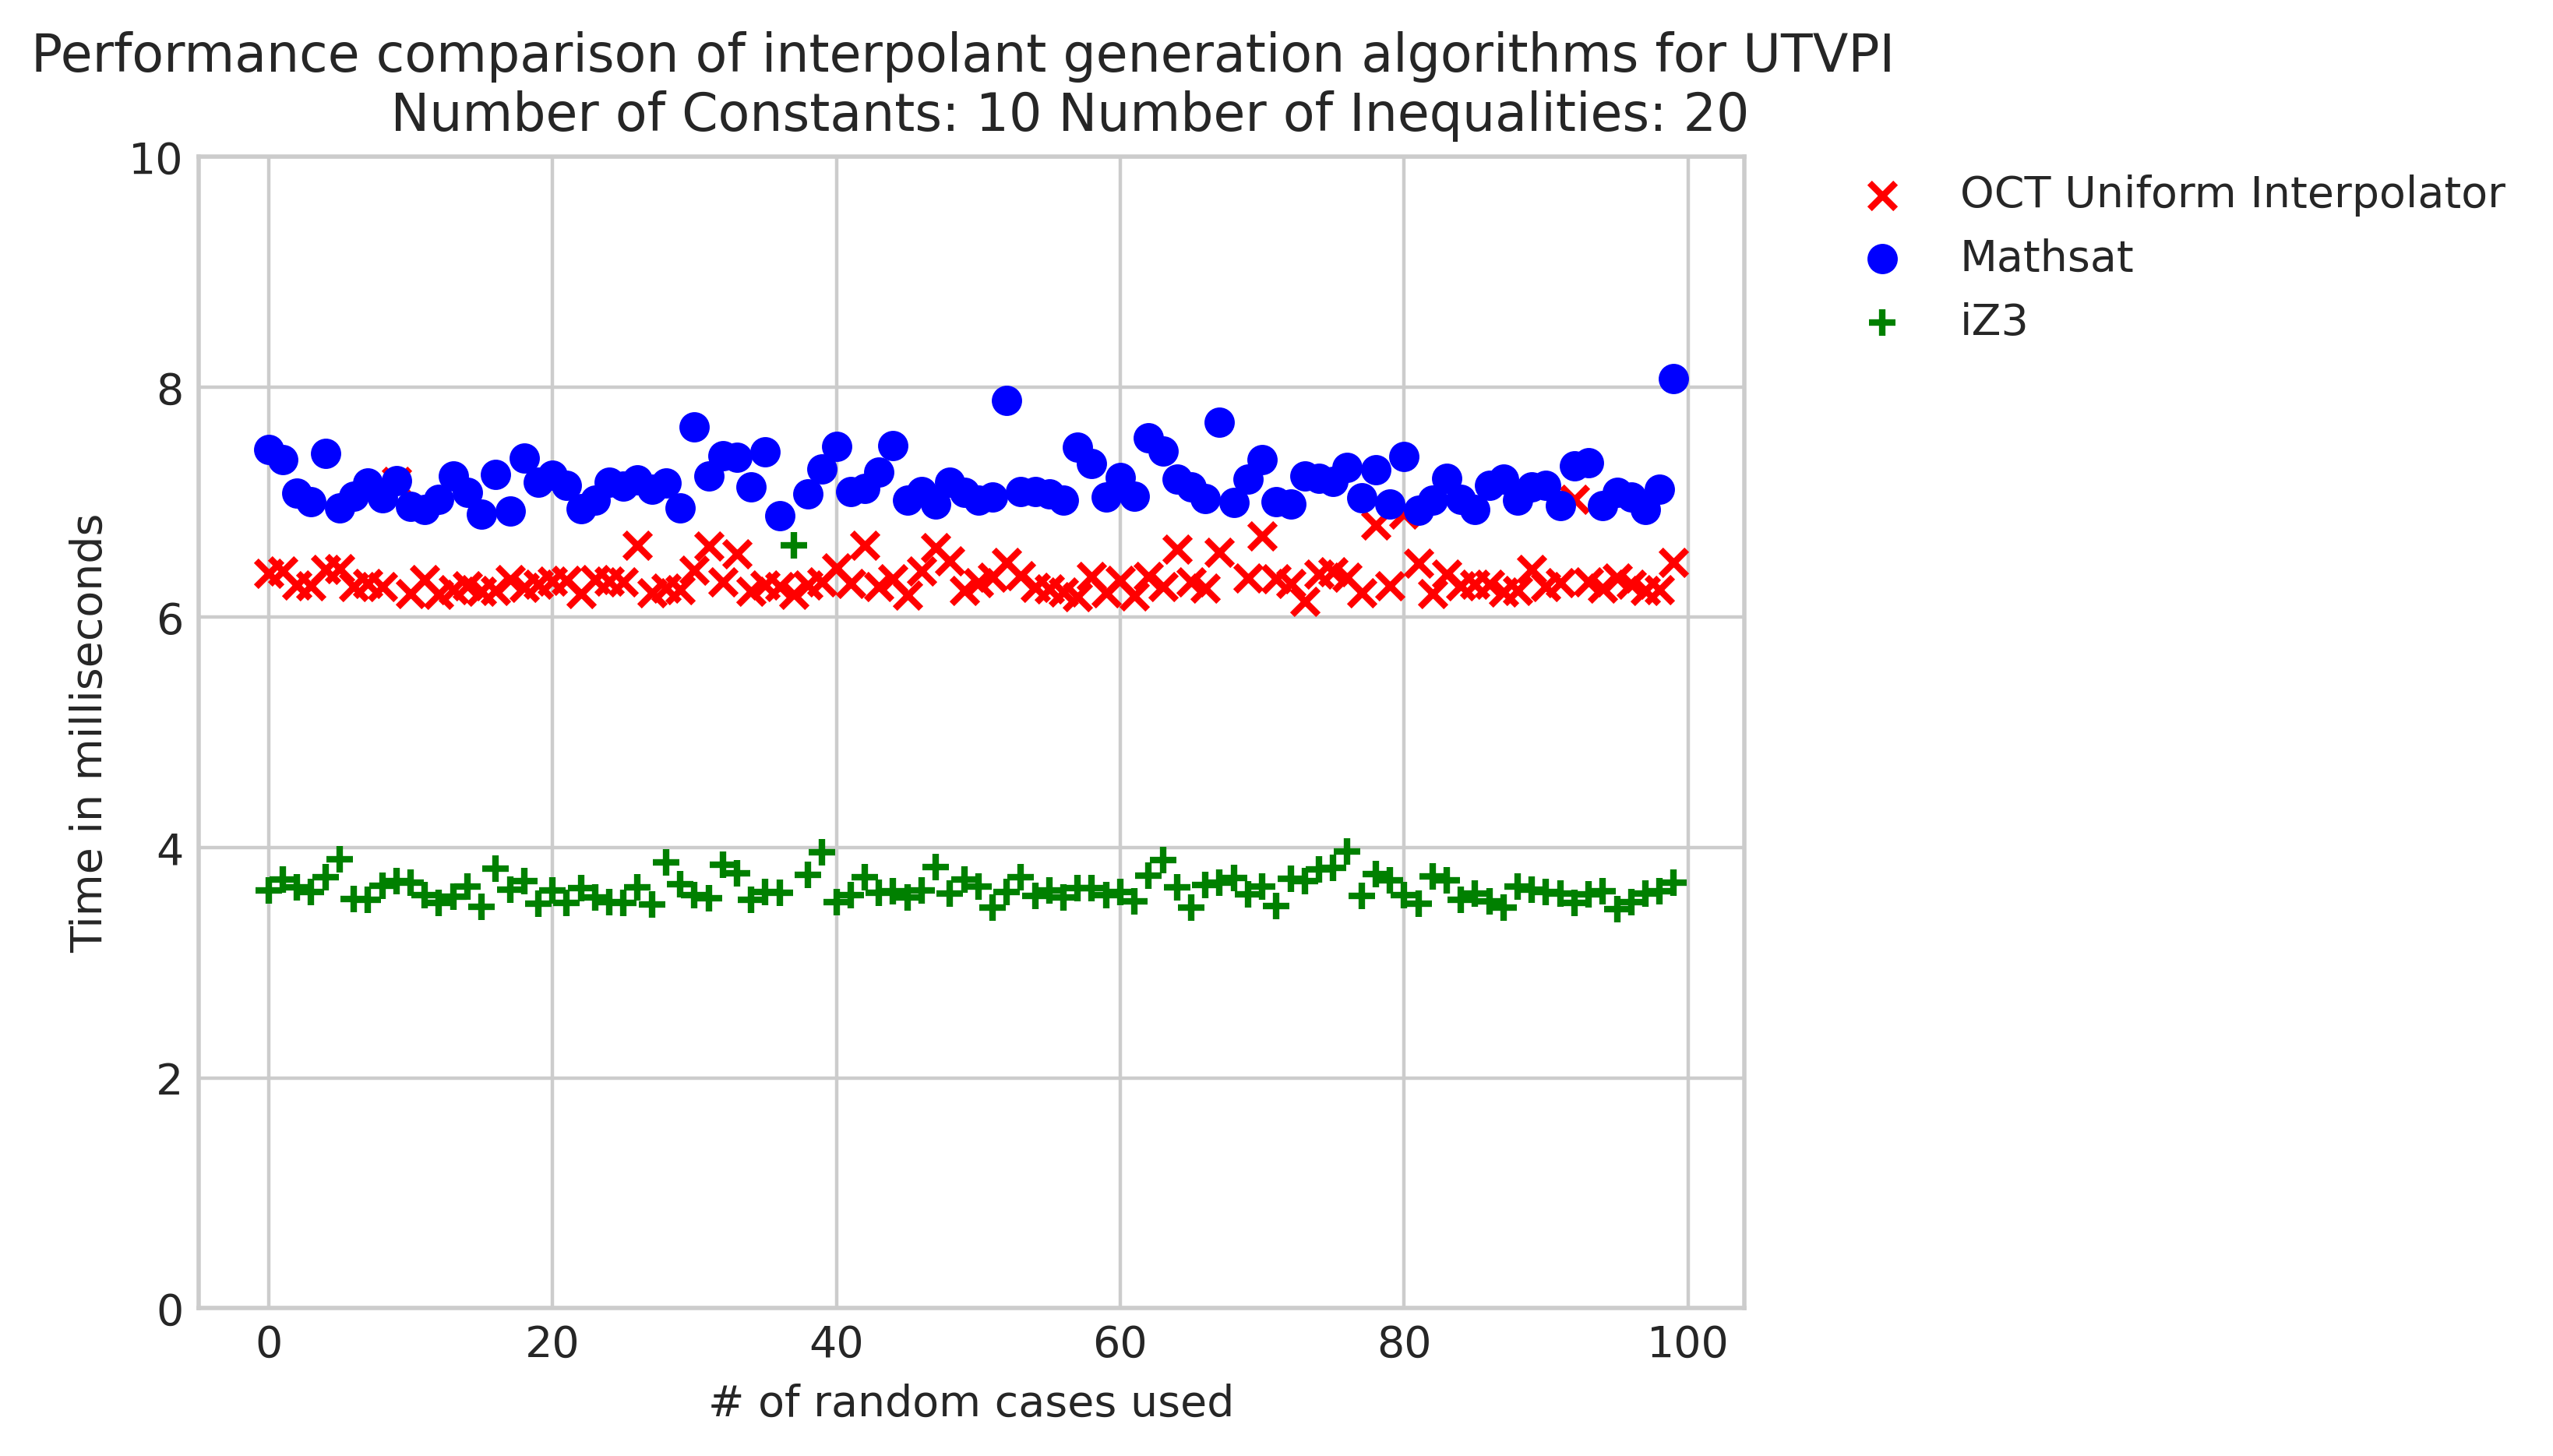
\includegraphics[scale=0.6]{figures/octi_performance_graph_10_20_100.png}
  \caption{Performance comparison graph of UTVPI interpolant generation
  algorithms for the benchmark (l = 1000, m = 10, n = 20)} 

  \label{performance_graph_oct_3}
\end{figure}

\begin{figure}
  \centering
  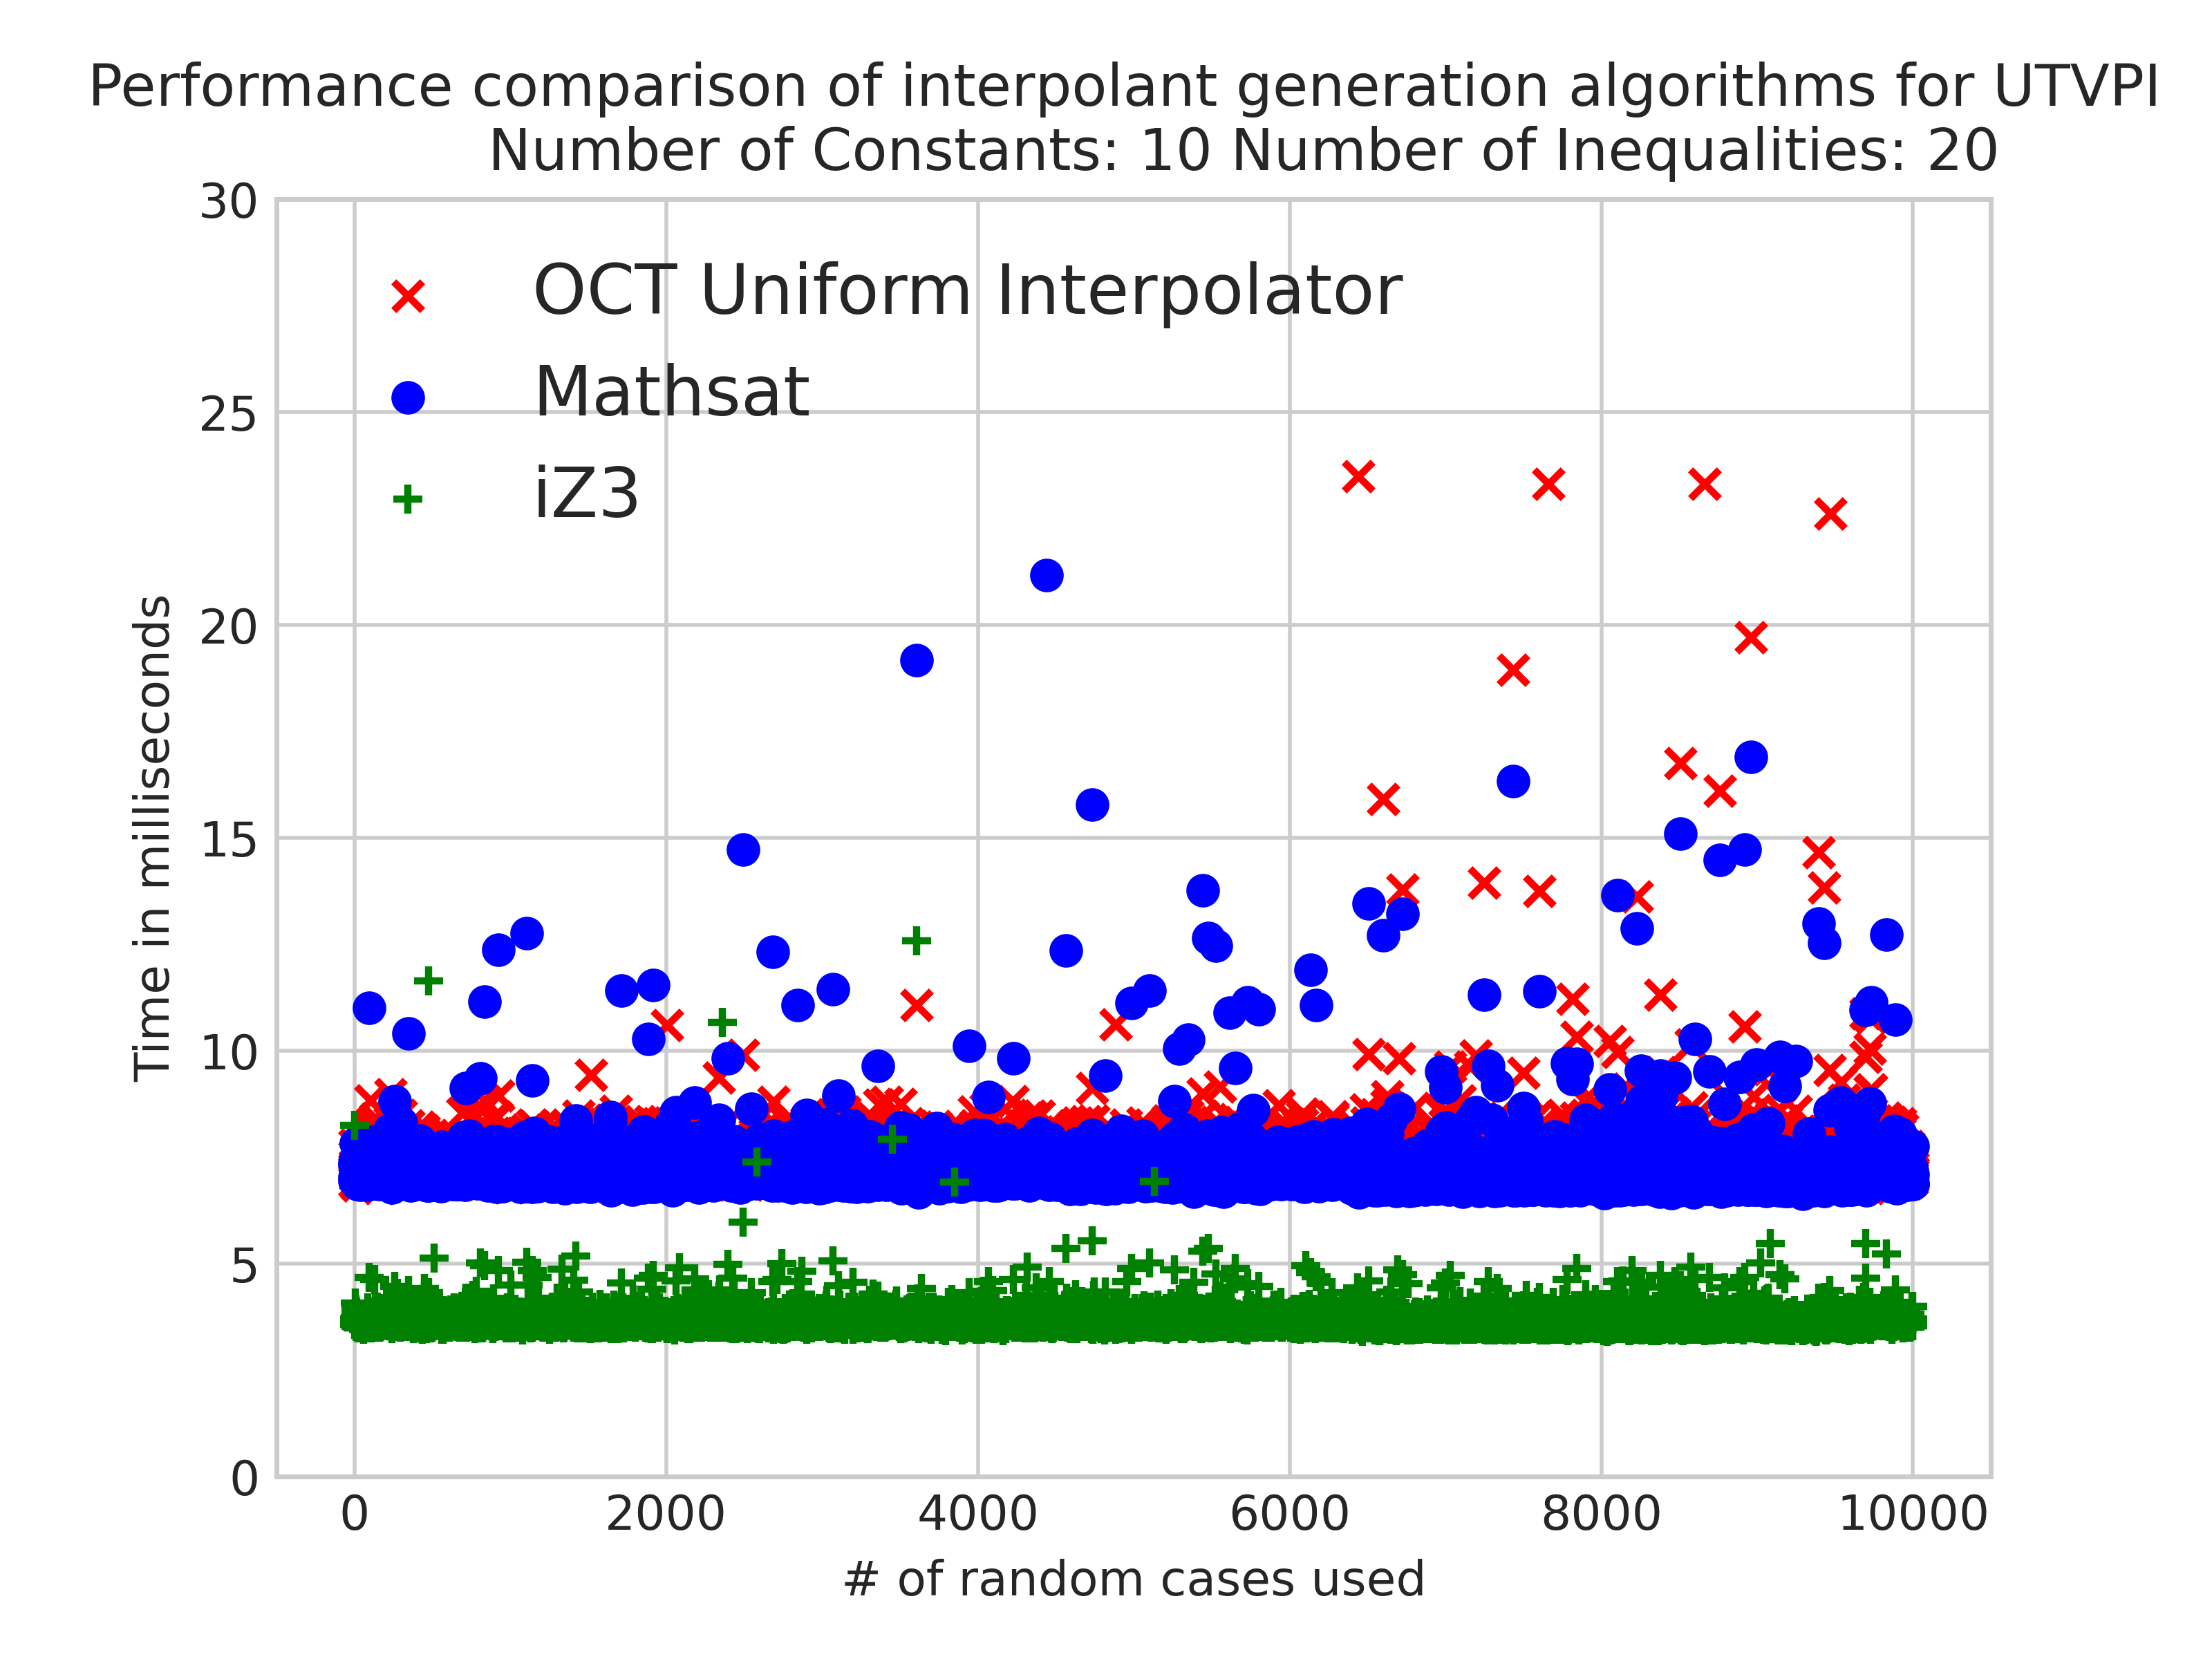
\includegraphics[scale=0.6]{figures/octi_performance_graph_10_20_10000.png}
  \caption{Performance comparison graph of UTVPI interpolant generation
  algorithms for the benchmark (l = 1000, m = 10, n = 20)} 

  \label{performance_graph_oct_4}
\end{figure}

%%% Local Variables:
%%% mode: latex
%%% TeX-master: "main"
%%% End:
